\documentclass[12pt]{scrartcl}

\usepackage[
  a4paper, mag=1000,
  left=2cm, right=1cm, top=2cm, bottom=2cm, headsep=0.7cm, footskip=1.27cm
]{geometry}

\usepackage[T2A]{fontenc}
\usepackage[utf8]{inputenc}
\usepackage[english,russian]{babel}
\usepackage{cmap}
\usepackage{amsmath}
\usepackage{tabularx}
\usepackage{array}
\usepackage{graphicx}
\IfFileExists{pscyr.sty}{\usepackage{pscyr}}{}
\usepackage[parfill]{parskip}
\usepackage{lastpage}
\usepackage{setspace} % single spacing between lines
\usepackage{blindtext} % for generated text - can remove
\usepackage{titlesec} % set header spacing
\setlength{\parindent}{15pt} % paragraph indent

\titlespacing{\section}{0pt}{\parskip}{-\parskip}
\titlespacing{\subsection}{0pt}{\parskip}{-\parskip}
\titlespacing{\subsubsection}{0pt}{\parskip}{-\parskip}

\usepackage[numbered]{bookmark}
\clubpenalty=10000
\widowpenalty=10000

\usepackage{fancybox,fancyhdr}
\pagestyle{fancy}
\fancyhf{}
\fancyhead[C]{\small{Олимпиадное программирование (средний уровень). Перебор --- день 01. \\ Летняя компьютерная школа ``КЭШ'', 8--28 августа 2017 года}}

%user-defined commands

\newcommand{\inputFile}{отсутствует}
\newcommand{\outputFile}{стандартный вывод}

\begin{document}

\singlespacing

\section*{Задача A. Разрушители сундуков}

\begin{tabularx}{\textwidth}{l l X}
    Имя входного файла: & \texttt{\inputFile} \\
    Имя выходного файла: & \texttt{\outputFile} \\
    Ограничение по времени: & $2$ секунды \\
    Ограничение по памяти: & $256$ мегабайт \\
\end{tabularx}

\begin{figure}[h]
	\centering
    
\includegraphics[width=0.6\linewidth]{Crashers.png}
\end{figure}

Красный, синий, зеленый и оранжевый рыцари во время погони за похищенными принцессами наткнулись на шайку разбойников. Между ними развязалась кровавая и ожесточенная битва, но рыцари в итоге смогли одолеть всех до единного.
В лагере разбойников, расположенном неподалеку от места стычки, они нашли сундук, спрятанный в кустах под огромной ивой. Но вот незадача, на сундуке был замок, ключ от которого мог быть где угодно. 
Опечаленные рыцари были готовы продолжить свой путь без сокровищ. Они подобрали свое оружие и собирались уже отправиться дальше, как их прервал низкий и немного сиплый голос. 
``Я знаю, где спрятан ключ, но за эту информацию я хочу попросить вашей помощи'' --- промолвил голос, исходивший от старой ивы. ``Чем мы можем вам помочь?'' --- спросил Синий рыцарь. 
``Если вы сообщите мне все числа от 100 до 1000, у которых вторая цифра равна 3 и который делятся без остатка на 5, то я отдам вам заветный ключ.''. \
Рыцари были очень талантливыми убийцами и магами, но совершенно ничего не смыслили в числах и математике. Помогите рыцарям решить поставленную перед ними задачу 

\subsection*{Формат выходных данных}
Выведите каждое число, соотвествующее условию задачи, на отдельной строке.

\newpage

\section*{Задача B. Разрушители барьеров}

\begin{tabularx}{\textwidth}{l l X}
    Имя входного файла: & \texttt{\inputFile} \\
    Имя выходного файла: & \texttt{\outputFile} \\
    Ограничение по времени: & $2$ секунды \\
    Ограничение по памяти: & $256$ мегабайт \\
\end{tabularx}

\begin{figure}[h]
	\centering
    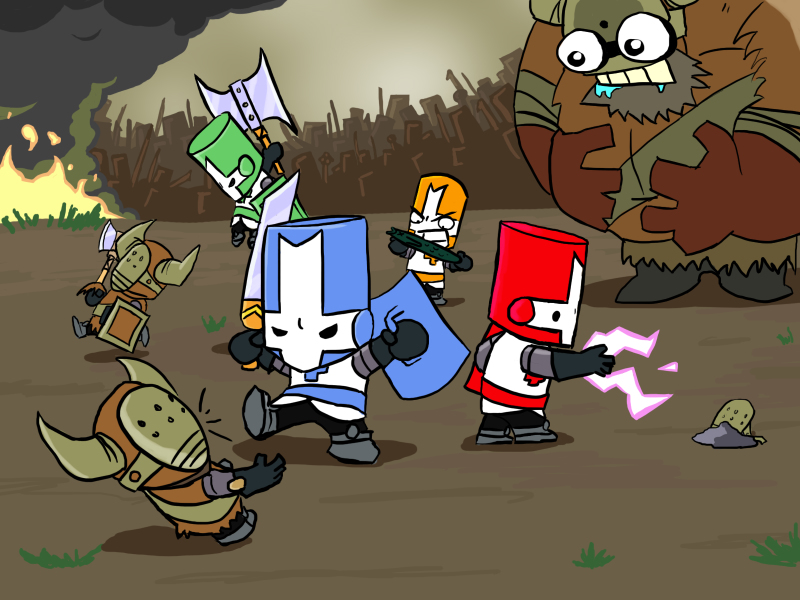
\includegraphics[width=0.6\linewidth]{Crashers2}
\end{figure}

Команда доблестных цветных рыцарей продолжила свой путь в замок волшебника, который нагло и бесцеремонно вломился в замок Короля и выкрал его дочерей и кристалл власти. 
По пути они храбро сражались с преспещниками волшебника, побеждая их один за другим. Спасательное путешествие привело их в пещеру Циклопа, но вход был закрыт магическим барьером.
Рыцари пытались сломать его силой, но ничего не получалось. Тогда Красный рыцарь, который знал магию лучше своих товарищей, достал книгу по волшебным барьерам из своего походного мешка и  
начал искать хоть какую-нибудь информацию, которая могла бы им помочь. Он читал, читал, читал, и наконец, он понял, как им пробраться внутрь. Тогда он радостно рассказал свою идею остальным.
Она заключалась в следующем: необходимо было последовательно высечь на барьере магические числа, а магическими числами назывались те, которые обязательно оканчивались на 5, а 2 и 3 цифра их сложенные вместе давали 7. 
Помогите рыцарям не пропустить ни одного магического числа, ведь иначе им придется начинать все сначала через день. 

\subsection*{Формат выходных данных}
Выведите каждое число, соотвествующее условию задачи, на отдельной строке.

\newpage

\section*{Задача С. Смертельный ребус Хетти}

\begin{tabularx}{\textwidth}{l l X}
    Имя входного файла: & \texttt{\inputFile} \\
    Имя выходного файла: & \texttt{\outputFile} \\
    Ограничение по времени: & $2$ секунды \\
    Ограничение по памяти: & $256$ мегабайт \\
\end{tabularx}

\begin{figure}[h]
	\centering
    
\includegraphics[width=1\linewidth]{Cat}
\end{figure}

На далеком-далеком острове в глубоком-глубоком океане стоял старый и уже изрядно обветшалый театр. С виду он мог показаться заброшенным, но это было далеко не так...

Однажды группа веселых друзей во главе с Хетти Хеттингтоном отправилась в морское путешествие на лодке ``Дружба'', но вечером они попали в ужасный шторм и кораблик потерпел крушение у острова, о котором никто не знал.
Все чудом спасенные (а спасенные ли?) друзья во главе с Хетти лежили без чувств на берегу таинственного острова. О, лучше бы они утонули, так как здесь их ждала участь намного-намного хуже...

Когда друзья очнулись, они обнаружили, что лежат в сырой и холодной камере, окруженные странными огромными котами в костюмах и шляпах. Но самое ужасное --- среди них не было всеми любимого Хетти!
Один из друзей, назовем его ``Безрассудный'', попытался поговорить с тюремщиками, но коты продолжали просто таращиться на них и пугающе молчать. Друзья сели обнявшись и стали ждать своей участи. 
Ближе к вечеру раздался громкий голос Хетти: ``Дорогие друзья, я хочу сыграть с вами в игру. Вам необходимо решить для меня одну маленькую задачку. Решите смертельный ребус: КТО+КОТ=ТОК, 
а если вы не успеете это сделать за 10 минут, то эти прекрасные коты пустят через камеру будоражущий мозг ток. Приступайте, друзья мои!'

Помогите друзьям избежать ужасной участи быть поджаренными высоким напряжением, а для этого решите за них заданный Хетти Хеттингтоном смертельный ребус.

\subsection*{Формат выходных данных}
Выведите каждое решение ребуса на отдельной строке, если их будет несколько.
Решение выводится в виде верного равенства, соответствующего описанному ребусу,
в котором все буквы заменены цифрами.
 
\newpage

\section*{Задача D. Мохнатые билетики}

\begin{tabularx}{\textwidth}{l l X}
    Имя входного файла: & \texttt{\inputFile} \\
    Имя выходного файла: & \texttt{\outputFile} \\
    Ограничение по времени: & $2$ секунды \\
    Ограничение по памяти: & $256$ мегабайт \\
\end{tabularx}

\begin{figure}[h]
	\centering
    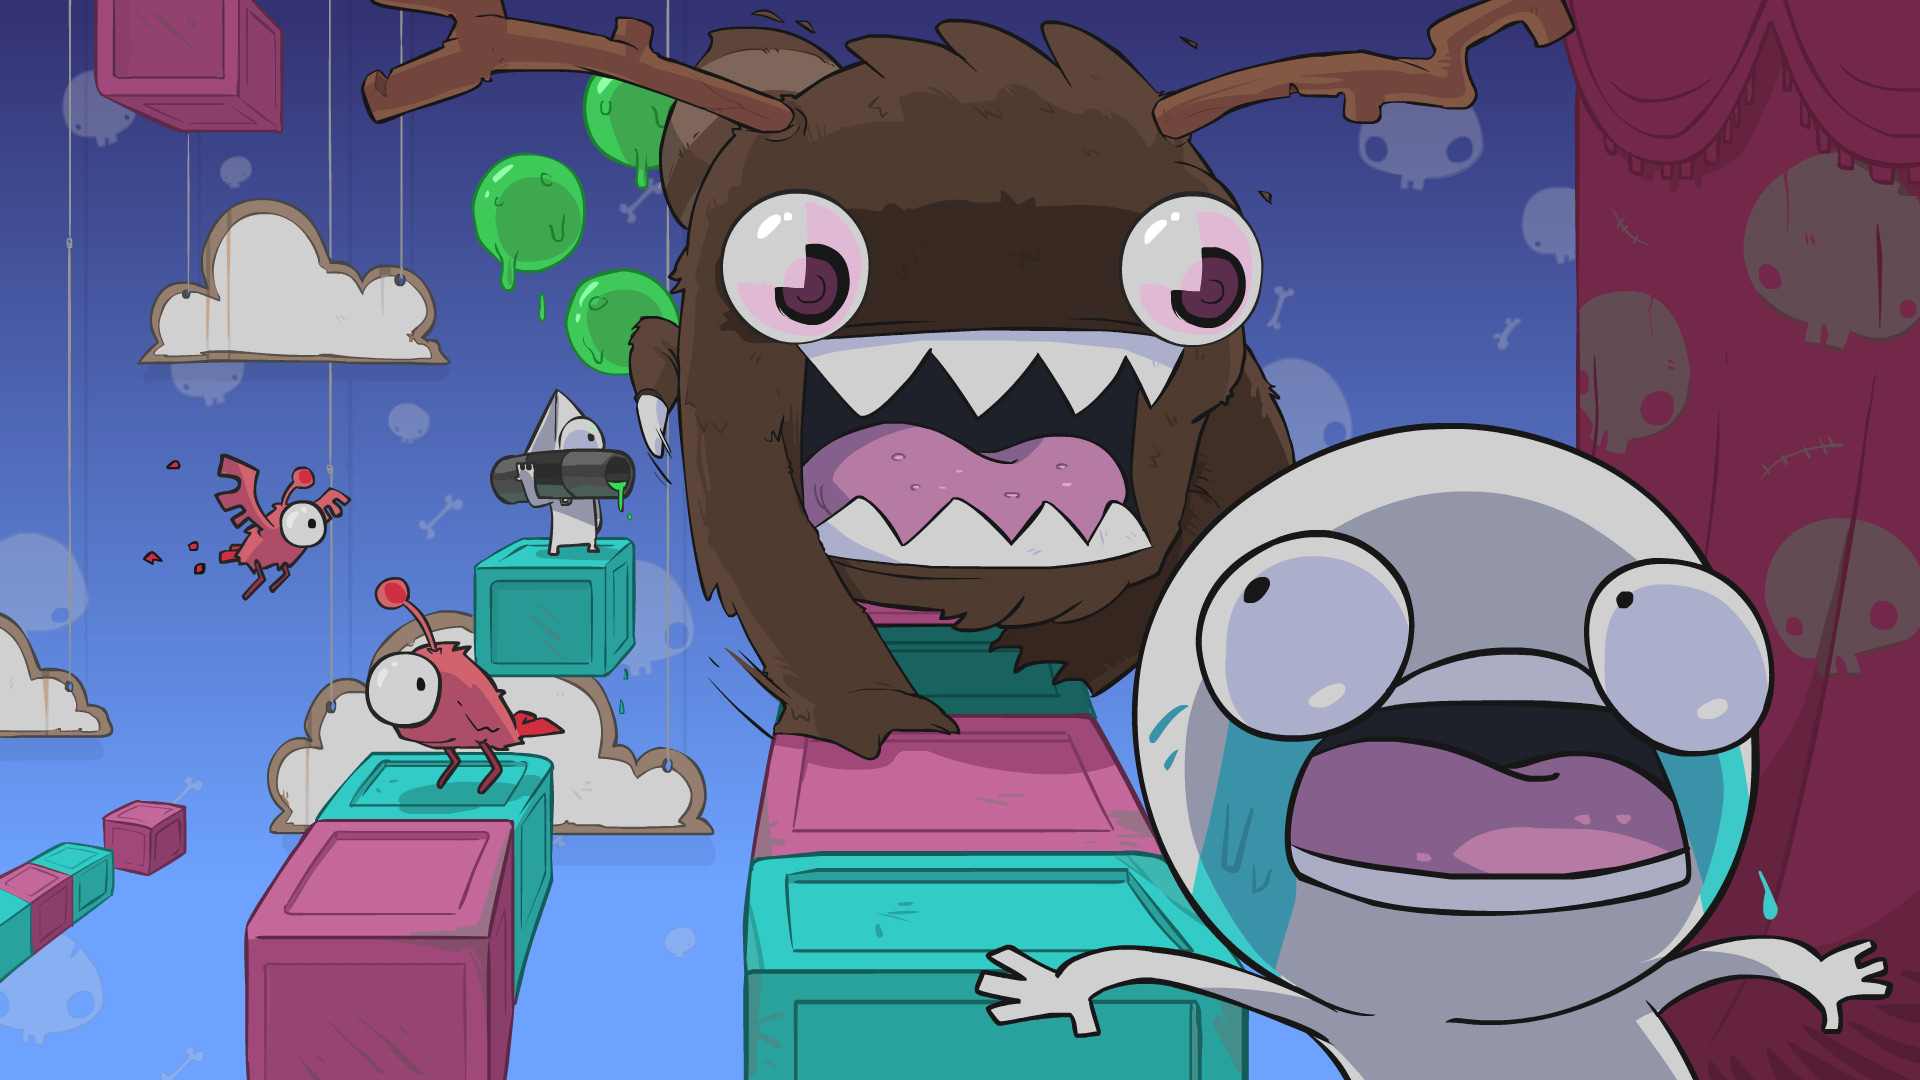
\includegraphics[width=0.8\linewidth]{tickets}
\end{figure}

\subsection*{Формат входных данных}

Хетти Хеттингтон часто устраивает для своих подручных котов волосатые гонки. 
Правила гонок очень просты --- один из заключенных в темнице друзей запускается на арену, состоящую из разнообразных препятствий,
и бедолаге необходимо попытаться выбраться, при этом собрав как можно больше пушистых оранжевых клубков по пути к выходу. При этом одним из препятствий является дружелюбный, 
но немного неуклюжий и вечно голодный монстрик, который очень хочет поиграть, 
и иногда так увлекается, догоняя своего нового убегающего и громко кричащего друга, что совершенно случайно, заглатывает его в свой бездонный желудок. 


Коты Хетти очень любят смотреть, как заключенные
справляются с испытанием-Мохнатиком (именно так они называют монстрика между собой), но этот участок арены доступен к просмотру не всем, а только счастливчикам, 
которым достанутся мохнатые билеты. 

Мистер Кот очень хочет посмотреть на мохнатое испытание, но он все время покупал не те билеты. В этом году он узнал, 
что оказывается у мохнатых  особый номер, а именно первые его три цифры с сумме дают то же число, что и три последние цифры числа. Он очень хочет выяснить номера билетов, которые обязательно окажутся мохнатыми. 


Помогите Мистеру Коту узнать номера всех мохнатых билетов, чтобы он наконец посмотрел на столь желанное им зрелище. 


\subsection*{Формат выходных данных}

Выведите все шестизначные числа, удовлетворяющие вышеизложенному условию. Каждое следующее число выводите с новой строки.

\newpage


\section*{Задача E. ЫЫЫЫЫЫ!}

\begin{tabularx}{\textwidth}{l l X}
    Имя входного файла: & \texttt{\inputFile} \\
    Имя выходного файла: & \texttt{\outputFile} \\
    Ограничение по времени: & $2$ секунды \\
    Ограничение по памяти: & $256$ мегабайт \\
\end{tabularx}

\begin{figure}[h]
	\centering
    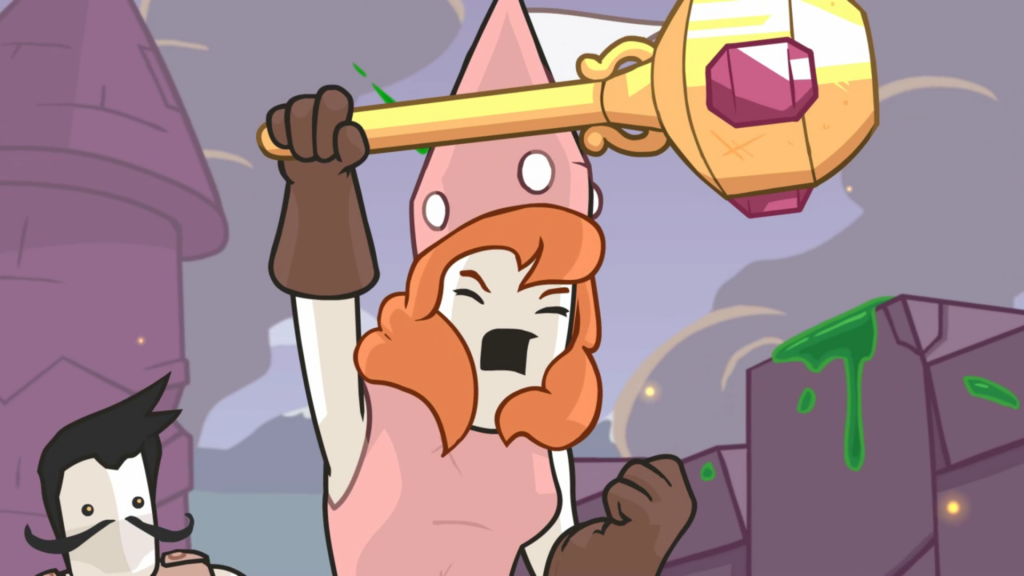
\includegraphics[width=0.5\linewidth]{yyyyy2}
\end{figure}

-Пипа попипапо пипипапопапа попипипопипипопапапо!

-Ыыовоаууфапввап абдурфвпрфыууууу...

-Попи?

-Арррааррр рарараррррр!
 
 \begin{equation*}
  \text{ТРИ + ТРИ + ТРИ = ДЫРА}
\end{equation*}

- ыыыЫЫЫЫЫ??? Та тарататата пауаамвла щощоу!
 
\begin{equation*}
  \text{(Ы + Ы) / Ы = Ы }
\end{equation*}

- Апаарапапа укточпарампампам!

\subsection*{Формат выходных данных}

{
\textbf{I SAID --- HORATIO DIES. KILL THEM, KILL THEM ALL!} 
}

{
\tiny Пробелы не нужны!
}

\begin{figure}[h]
	\centering
    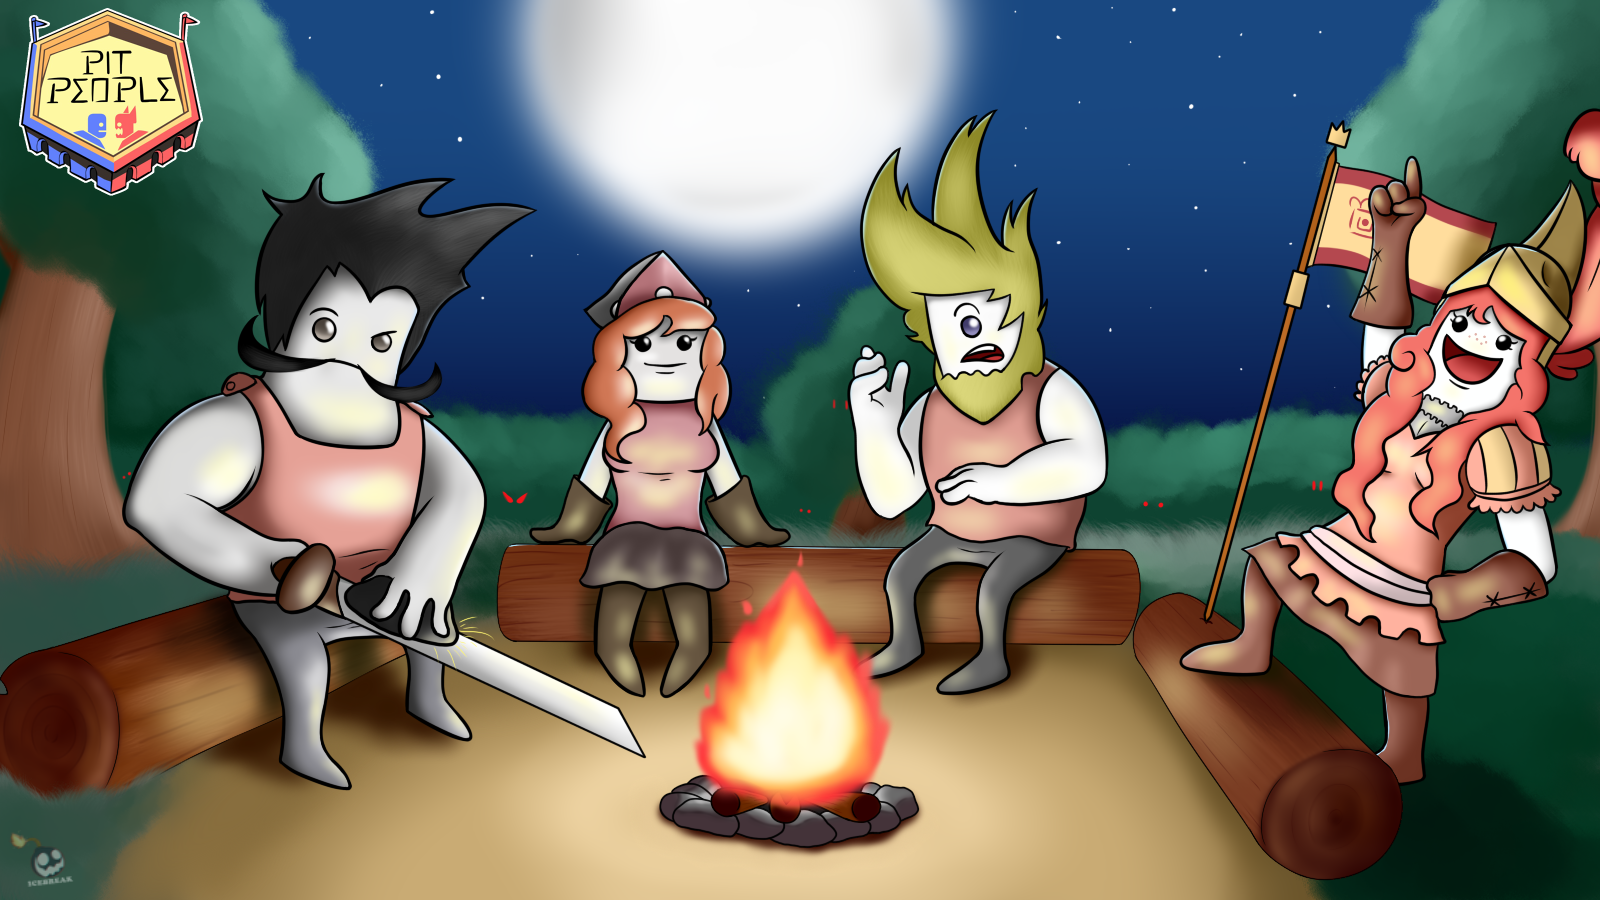
\includegraphics[width=0.6\linewidth]{yyyyyy!}
\end{figure}

\end{document}